\Chapter{EMAIL2GIT: FROM ACADEMIC RESEARCH TO OPEN-SOURCE SOFTWARE}\label{sec:Theme2}

As explained in \autoref{sec:Introduction}, the linux contribution process is a strong email-based system that has proven to be reliable and scalable over the years. Like in many other organizations, the linux development community makes extensive use of code reviews to ensure the quality of contributors' code submissions. These code reviews occur in the mailing lists, where the patch was first introduced. After accepting and integrating the patch to the git repository, it is usually very hard to recover the original patch, the code reviews, and the discussion that took place during the code reviews. 

Other tools, such as github and gerrit, have addressed this issue by providing a code review environment and by keeping track of the code review for each commit. However, these environments often do not broadcast the code reviews to everyone. These \textit{unicast} review environments only notify the author to read the code reviews by default. In a quantitative study, \citep{armstrong} examined the differences between \textit{unicast} and \textit{broadcast} review system. The authors discovered that broadcast allows for faster review cycle, and provides learning material for new developers. The linux community never used these tool for upstream contributions as they would not scale to the size of the linux community. 


Since the kernel's mailing list-based review process is here to stay, we instead address the lack of way to backtrack reviews, we implemented Email2git. The tool is able to find, for a given linux commit, the original patches and the code reviews. This chapter introduce Email2git, from its inception, to its deployement to production. 

\section{Previous Publications and Original Algorithm}

The original algorithm capable of backtracking patches from commits was introduced in two papers~\citep{msr13jojo,jiang14} published by Jiang, a former member of the MCIS Lab.

The ultimate goal of the algorithm is to find the patch or patches that introduced a single commit. To do that, Jiang creates a SQLite database containing all the patches extracted from the mailing lists. This database contains each patch's +/- lines. The script will then parse a dataset containing all the git commits and find corresponding patches in the database. More specifically, the script queries the database for patches containing the same +/- line contained in each commit. The algorithm then ranks the possible matches by the proportion of lines in common between the commit and the patch. It is important to understand that a patch may have undergone several rounds of reviews before being committed. This means that a single commit will likely be matched to multiple patches. 

% The general idea of the algorithm was to compare the +/- lines from both the accepted version of a patch and the email patches at the time of the review. A match was found if the proportion of identical +/- lines was above a certain threshold. 

Although this script was a great proof of concept, I was not able to scale it on our 8-year-long dataset. Hence, we designed and implemented a new algorithm based on the original algorithm capable of scaling to larger dataset. This new implementation is described in \autoref{sec:scaling}.

% For example, there are 5 +/- lines in a commit $A$'s diff. The algorithm iterates through the patches present in the dataset, comparing the 5 +/- lines form the commit to the +/- lines from each patch. To compare the +/- lines from the commits and the patches, the algorithm find the proportion of identical lines in both the commit and the patch. A patch will be matched to commit $A$ if the proportion of identical lines is above a certain threshold. 



\section{Scaling the Algorithm}
\label{sec:scaling}

Since we had access to email patches dating back to 2009, we decided to extract git commits from the Linux git repository from the same date until the release of linux v4.11, which represent over \textit{500,000 commits} to analyse. Unfortunatly, this amount of data was too large for the orignal algorithm to parse in a timely fashion.

This called for a new, scalable algorithm that leverages the heuristics mentioned in \citep{msr13jojo,jiang14}.

We were able to separate the matching process into multiple different phases. After each phase, the matched commits and patches are removed from the dataset to reduce the workload for the next phase. The different phases are explained in this section. 

\begin{figure}[htb]
\centering
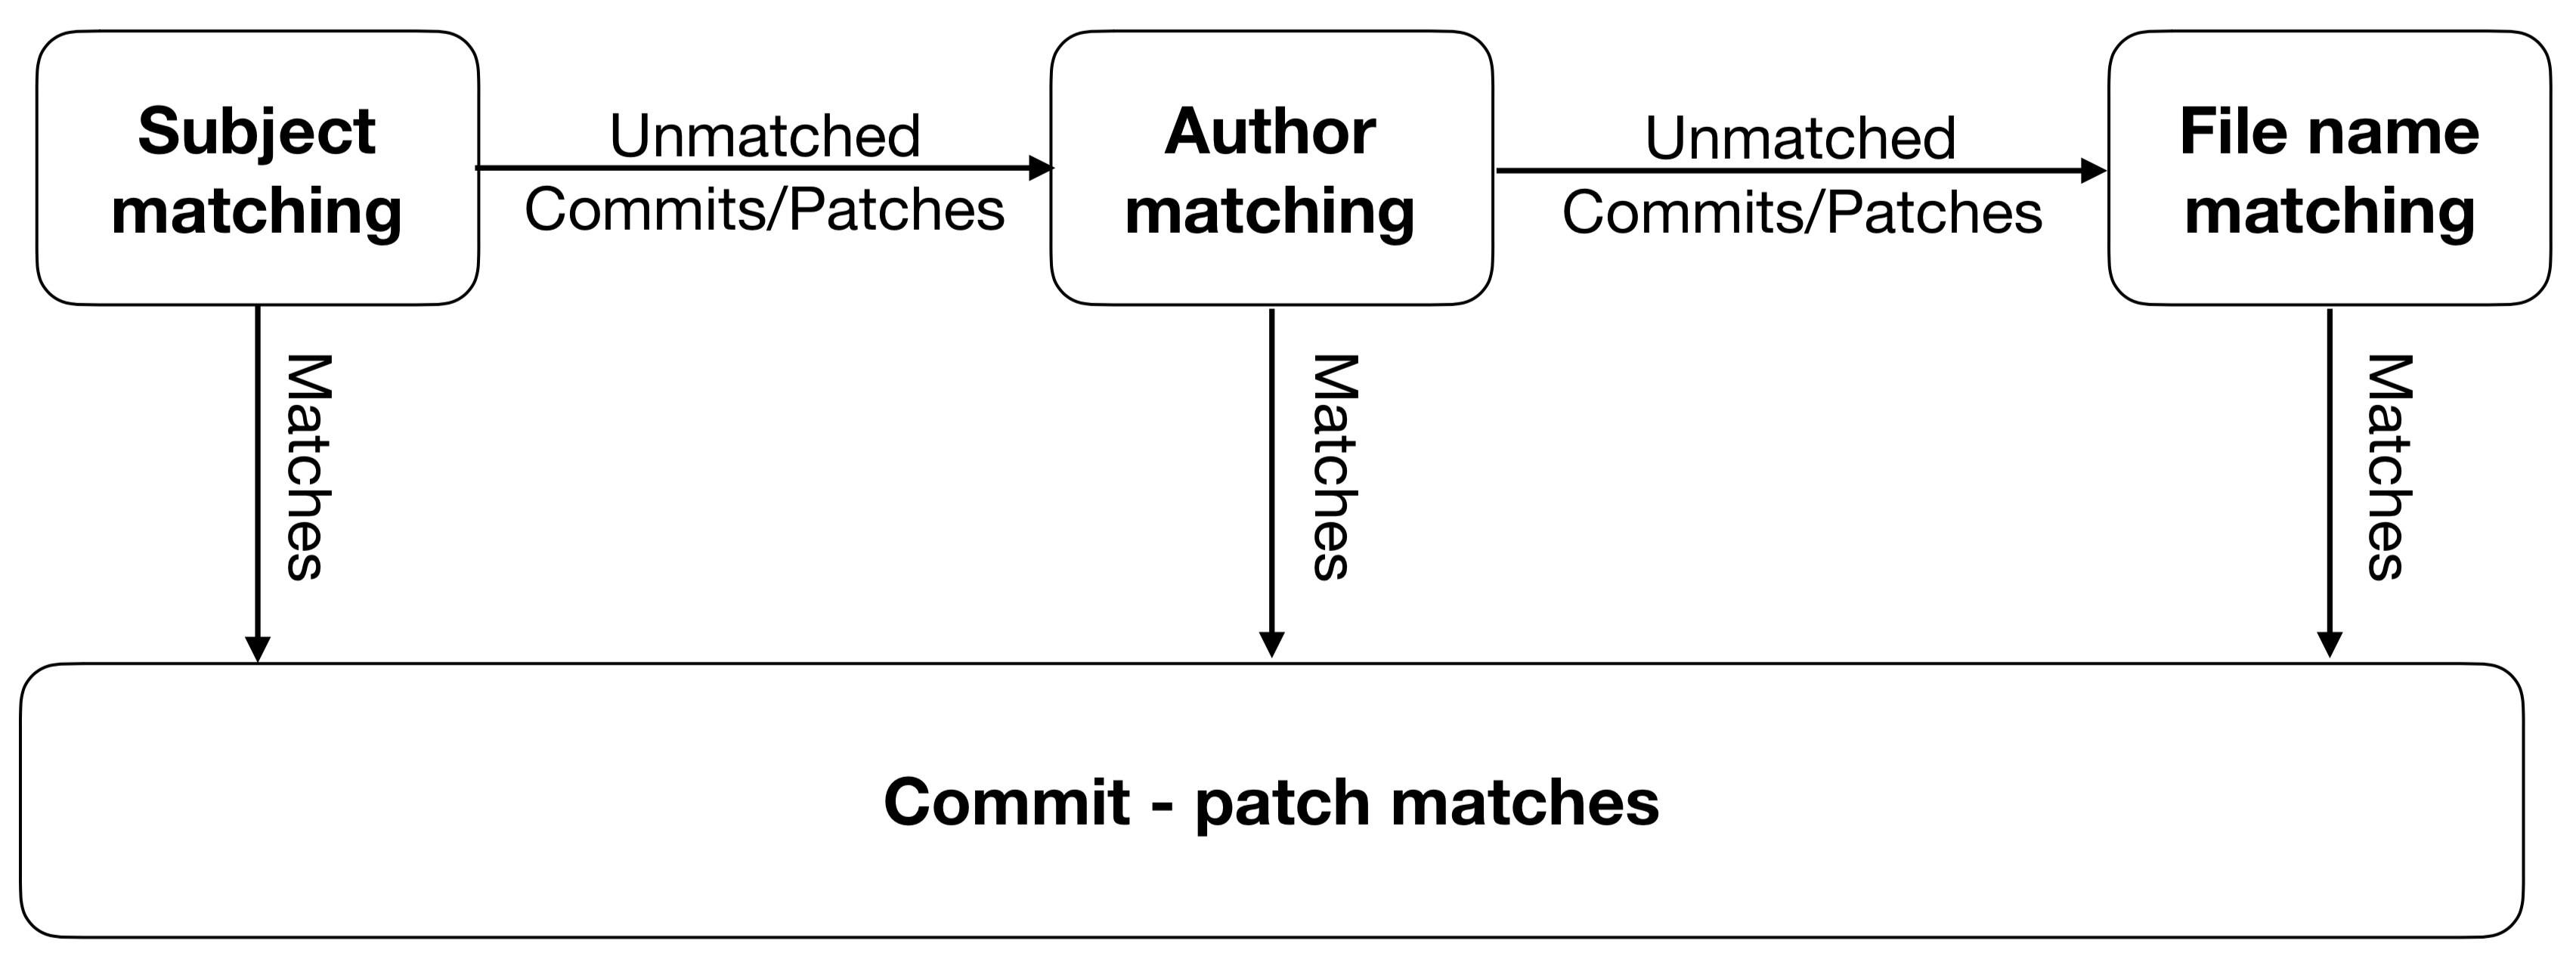
\includegraphics[width=5in]{new_algo_matching}
\caption{The three phases of the new algorithm}
\label{fig:new_algo_matching}
\end{figure}

\subsection{Patch Email Subject}

The most important heuristic that drastically increased the matching speed is the \textit{email subject - commit summary} concept. The built-in git feature \texttt{git format-patch} and \texttt{git send-email} allows developers to easily submit their changes to a maintainer by email according to the Linux Kernel Contribution guidelines\footnote{\url{https://kernelnewbies.org/FirstKernelPatch}}. The piece of information we are interested in is the email subject. \texttt{Git am} automatically saves the email subject and uses it the "commit summary". This commit summary, or commit title, is the first line of the commit message as explained in \autoref{sec:commit_anatomy}. Comparing both strings of characters allows for a very quick first phase of matching.

Jiang originally used the email subject as oracle to evaluate her original algorithm. We use it as the first phase of the new matching process. We then remove the matched commits and patches from the dataset to reduce the workload of the next steps.



\subsection{Author and Affected Files}

Even though the number of commits was reduced by half after the first phase, the remaining data was still too large to use brute force (comparing each commit against each patch). This is due to the time complexity of the script. For each commit to analyse, the script has to go through every patch in the dataset. Given a time complexity of $O(n^2)$, the time taken to execute the script increases quadratically as the size of the dataset increases. Thus, we had to find a way to use the available meta-data to speed up the matching. The first data point used was the \textit{author name}. As depicted in \autoref{fig:author_matching}, one can use the name and email address of the \textit{commit author} to pin point to the patches that were sent by the same person. In other words, to find a match for each commit, the algorithm has to parse a handful of patches (those by the same author as the commit) instead of hundreds of thousand. After a commit is pointed to a group of patches, it utilises the line-based algorithm used in the original script. Similarly, we use the same technique with the name of the files affected by a commit and a patch can to increase the performance of the +/- line algorithm. Through regular expression and text parsing, we can retrieve the files that are modified in the patch and the \textit{commit diff}. Since the author-based matching is slighty faster and returns more matches than the file-based matching, we start with the former, removing each matched commit and patch to reduce the workload of the next phase.

\begin{figure}[htb]
\centering
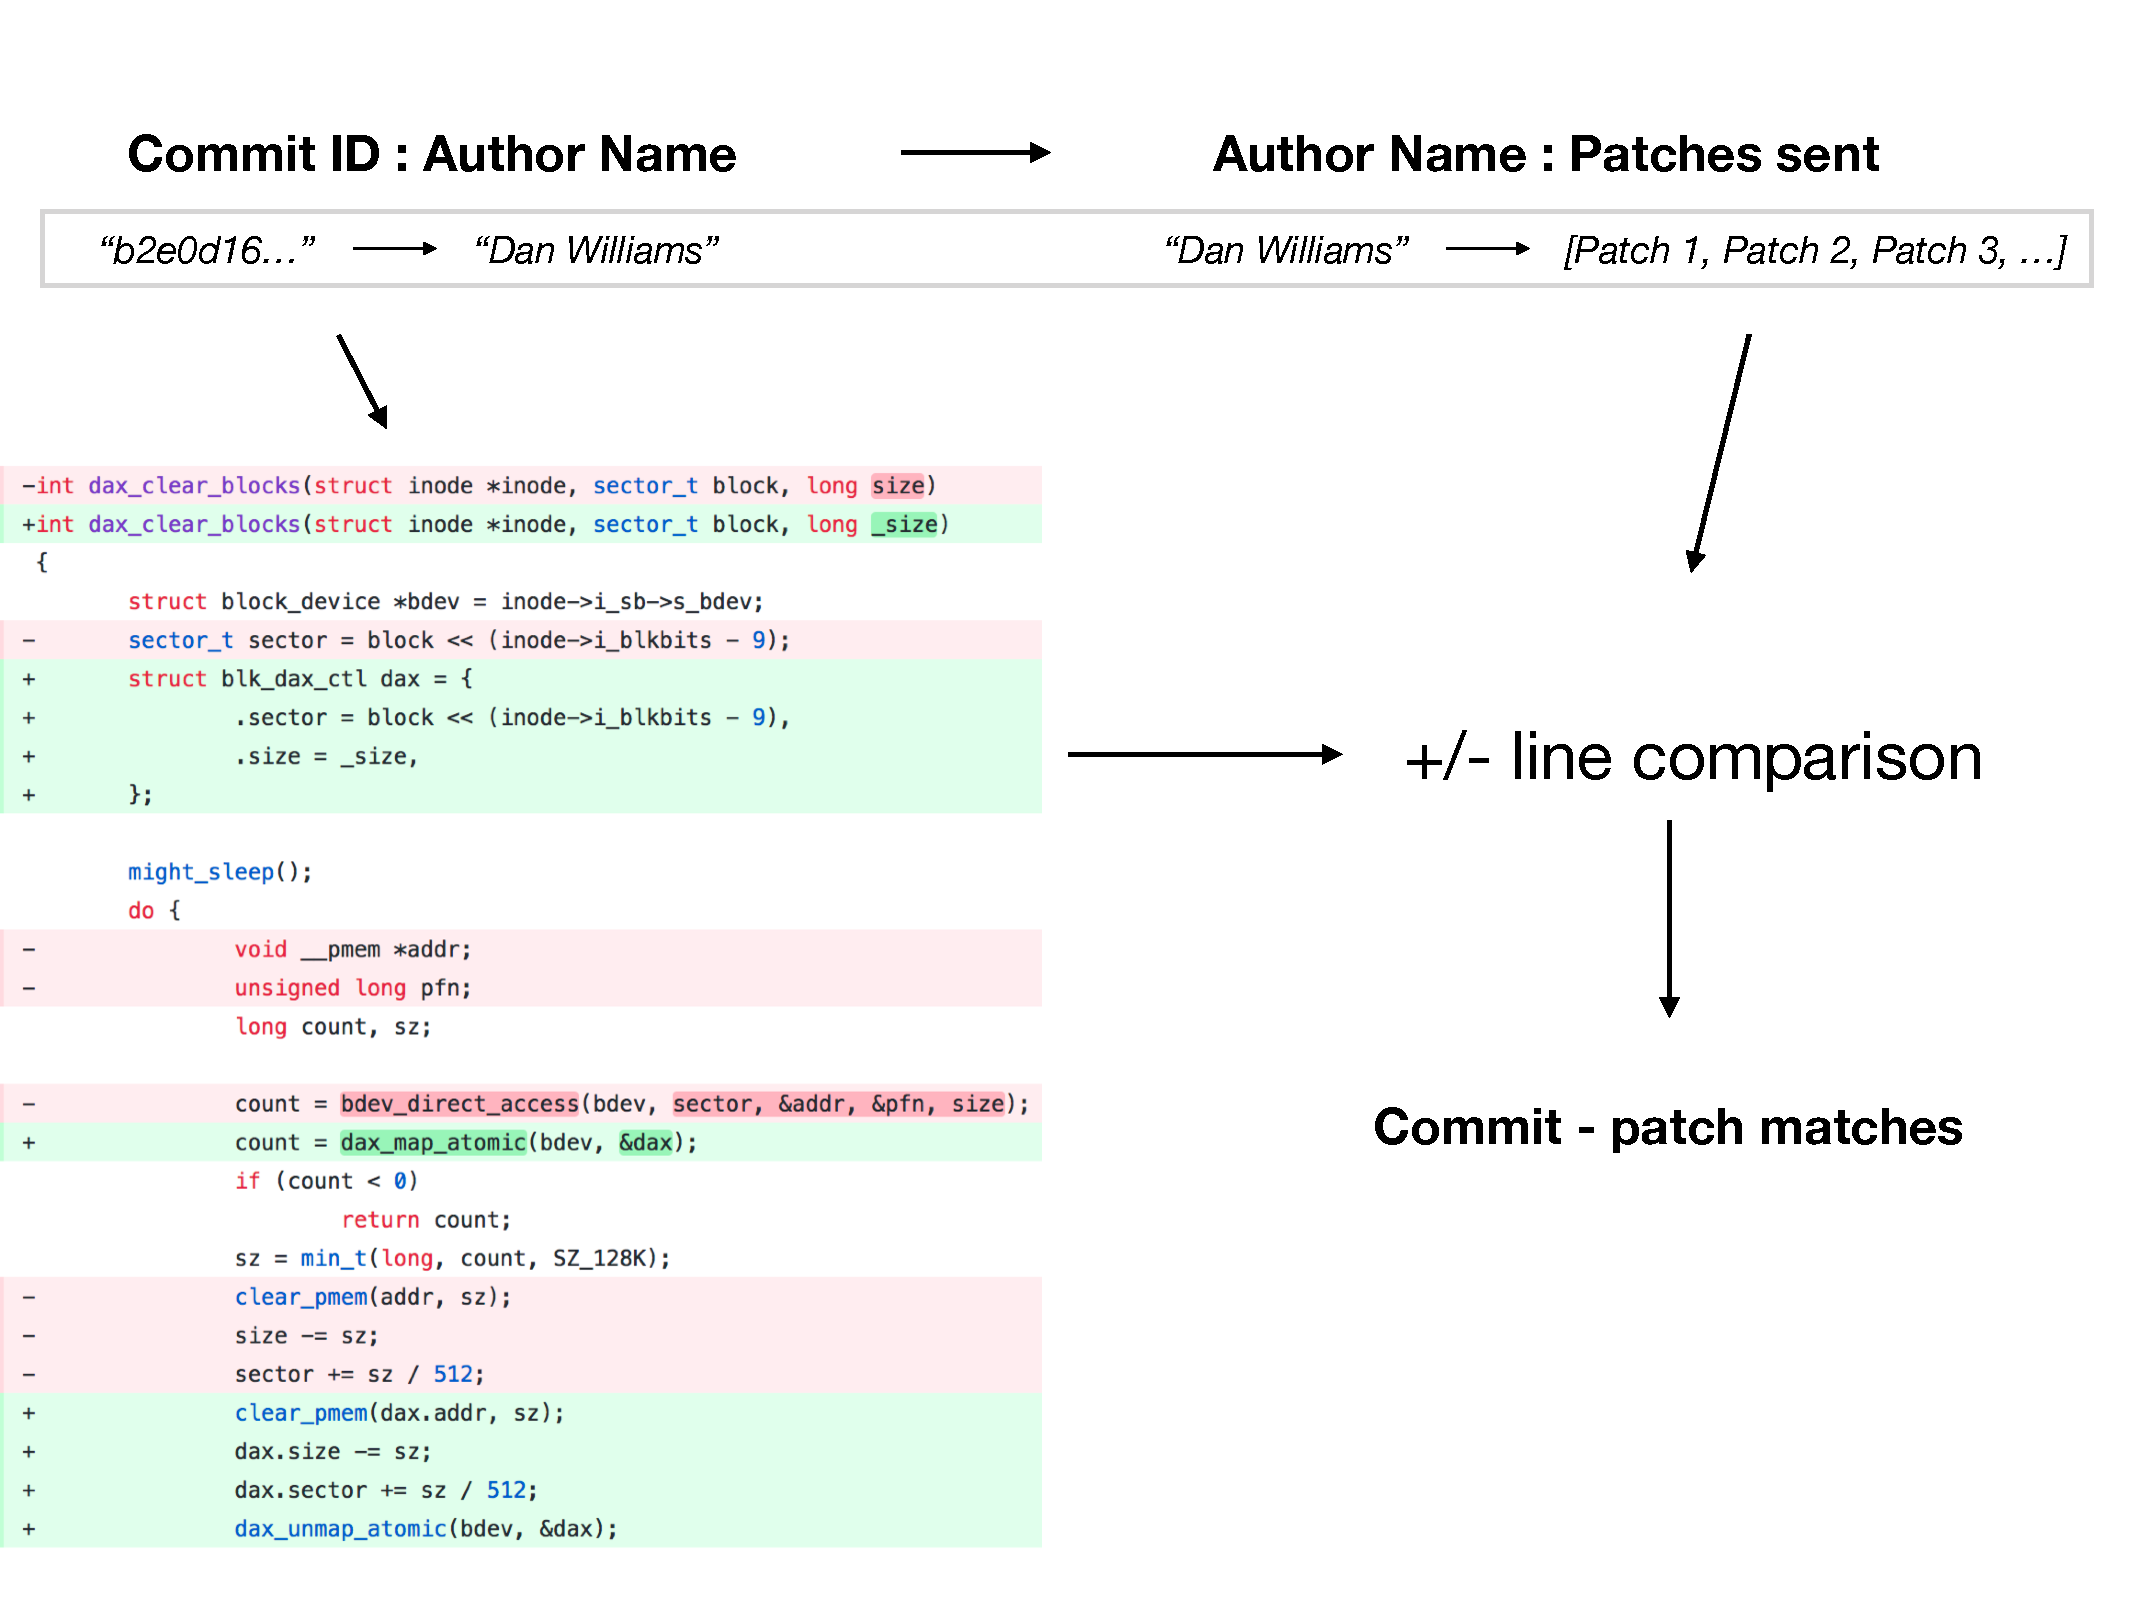
\includegraphics[width=5in]{author_matching_tmp}
\caption{Using the patch sender to assist matching}
\label{fig:author_matching}
\end{figure}


\section{The Data}

There are two sides to this matching process: the Linux git repository and the archives containing the patches sent in mailing lists over the years. We need to extract the diff (+/- lines), the metadata, and the subject and commit summary from both side. The scripts used for each part of the data extraction are available on the Email2git project's github under the GPL-3.0 license \footnote{\url{https://github.com/alexcourouble/email2git}}.

Because we wanted Email2git to be a usable and practical tool, we needed a way to display the patches and the code reviews in a browser. \textbf{Patchwork}\footnote{\url{https://github.com/getpatchwork/patchwork}} is a tool designed to assist maintainers of open source projects using an email-based contribution process. It tracks the mailing lists used by developers to submit patches and receive code reviews. The tool extracts each detected patch as well as its associated reviews, then displays them in a web-based user interface. Additionally, Patchwork stores the patches in a database, along side a unique ID that can be used to generate a URL to that patch.

We were granted read access to the MySQL database behind a patchwork instance hosted on kernel.org\footnote{\url{https://patchwork.kernel.org/}}. This instance has been tracking 69 of the many linux subsystems mailing lists since 2009, giving us the opportunity to analyse over \textit{1.4 million} patches.

In addition to being a data source, patchwork.kernel.org also represents a way for us to display the patches and the code reviews associated with commits to the users. The only limitation of this patchwork instance is that it does not track some major mailing lists, particularly some of the \texttt{Net} mailing lists.


\subsection{The Commits}

First, we need to extract the commit summary from each commit after 2009. This date is our lower bound because our email data from patchwork.kernel.org only has email patches dating back to 2009. The commit summary is the first line of the commit message, which makes it very easy to retrieve. The script \texttt{subject\_data\_gen/commit\_subject\_generator.py} reads a git log output and stores the commit summary for each commit in a SQLite3 database. The exact git log command used is the following:
\begin{lstlisting}
git log --no-merges --pretty=format:"%H,%ct,%s" --after={2009-01-01}
\end{lstlisting}
The \texttt{pretty} option formats the output according to the passed parameters. 

The next step on this side of the data is to extract the data for the other phases of the matching process. The script \texttt{lines\_data\_prep/git\_prep.py} is more complicated, as there is more data to parse and save. This script reads the authors and the files affected by each commit. It will then create two maps: commit ID to author, and commit ID to files affected. These maps, which exist as python dictionaries are then saved to two separate pickle files\footnote{\url{https://docs.python.org/2/library/pickle.html}}, which make writing, reading, and storing data fast and easy. This script also extracts the +/- lines from the commit diff and stores them in a pickle file as well. 



\subsection{The Patches}

The patches are stored on a remote serve in a MySQL database, the same database that hosts the patchwork.kernel.org data. Through the help of SQL queries, I dumped all the necessary data in csv files to avoid complications arising from handling a production database. Once those csv files created, I could parse them with the help of two python scripts available in the Email2git githubg repository. \texttt{subject\_data\_gen/patchwork/pwSubjectFull.py} takes care of the subject data and \texttt{lines\_data\_prep/pw\_prep.py} takes care of the authors, file names, and +/- lines of the patches. Here again, the subject data is stored in a SQLite3 database, and the line data is stored in pickle files. 







\section{Providing Access to the Matches} 

Now that matches have been generated and saved, we need a way to make the information available to linux developers. Each match is composed of four elements: the \textit{commit ID}, the \textit{patchwork permalink ID}, the \textit{date}, and the \textit{phase} that found the match (subject, author, or file). The patchwork permalink ID is used to point to the patch and conversation on patchwork.kernel.org.

Email2git's original intended contribution was to increase the amount of information available in Srcmap by providing access to the conversation that took place during the creation of the patch. However, since cregit was more popular than Srcmap, we decided to integrate Email2git with Cregit instead. Additionally, we made our data available through a standalone commit lookup interface.

\subsection{Integrating Email2git with Cregit}

Cregit is a project that aims at providing a finer grained approach to \textit{git blame}. The blame option in git returns the name of the developer who last changed a line of code in the source code. It provides a way to quickly unmask the developers responsible for code in the source code. However, it has a serious limitation: git blame assigns a line to a developer even after a small modification to that line. For instance, if developer $A$ writes \texttt{print "Hello world"}, this line will then become associated with developer $A$. However, if developer $B$ modifies the line to read \texttt{print "Hello world!"}, git blame will associate the line with devloper $B$ even though developer $B$ only added a character. 

Cregit addresses this limitation by tokenizing the source code in a git repository to enables git blame at a token level, instead of a line level. This provides a better understanding of the true authors of the source code. A tokenized version of the Linux kernel source code is available online through the cregit interface\footnote{\url{https://cregit.linuxsources.org/}}.

\begin{figure}[htb]
\centering
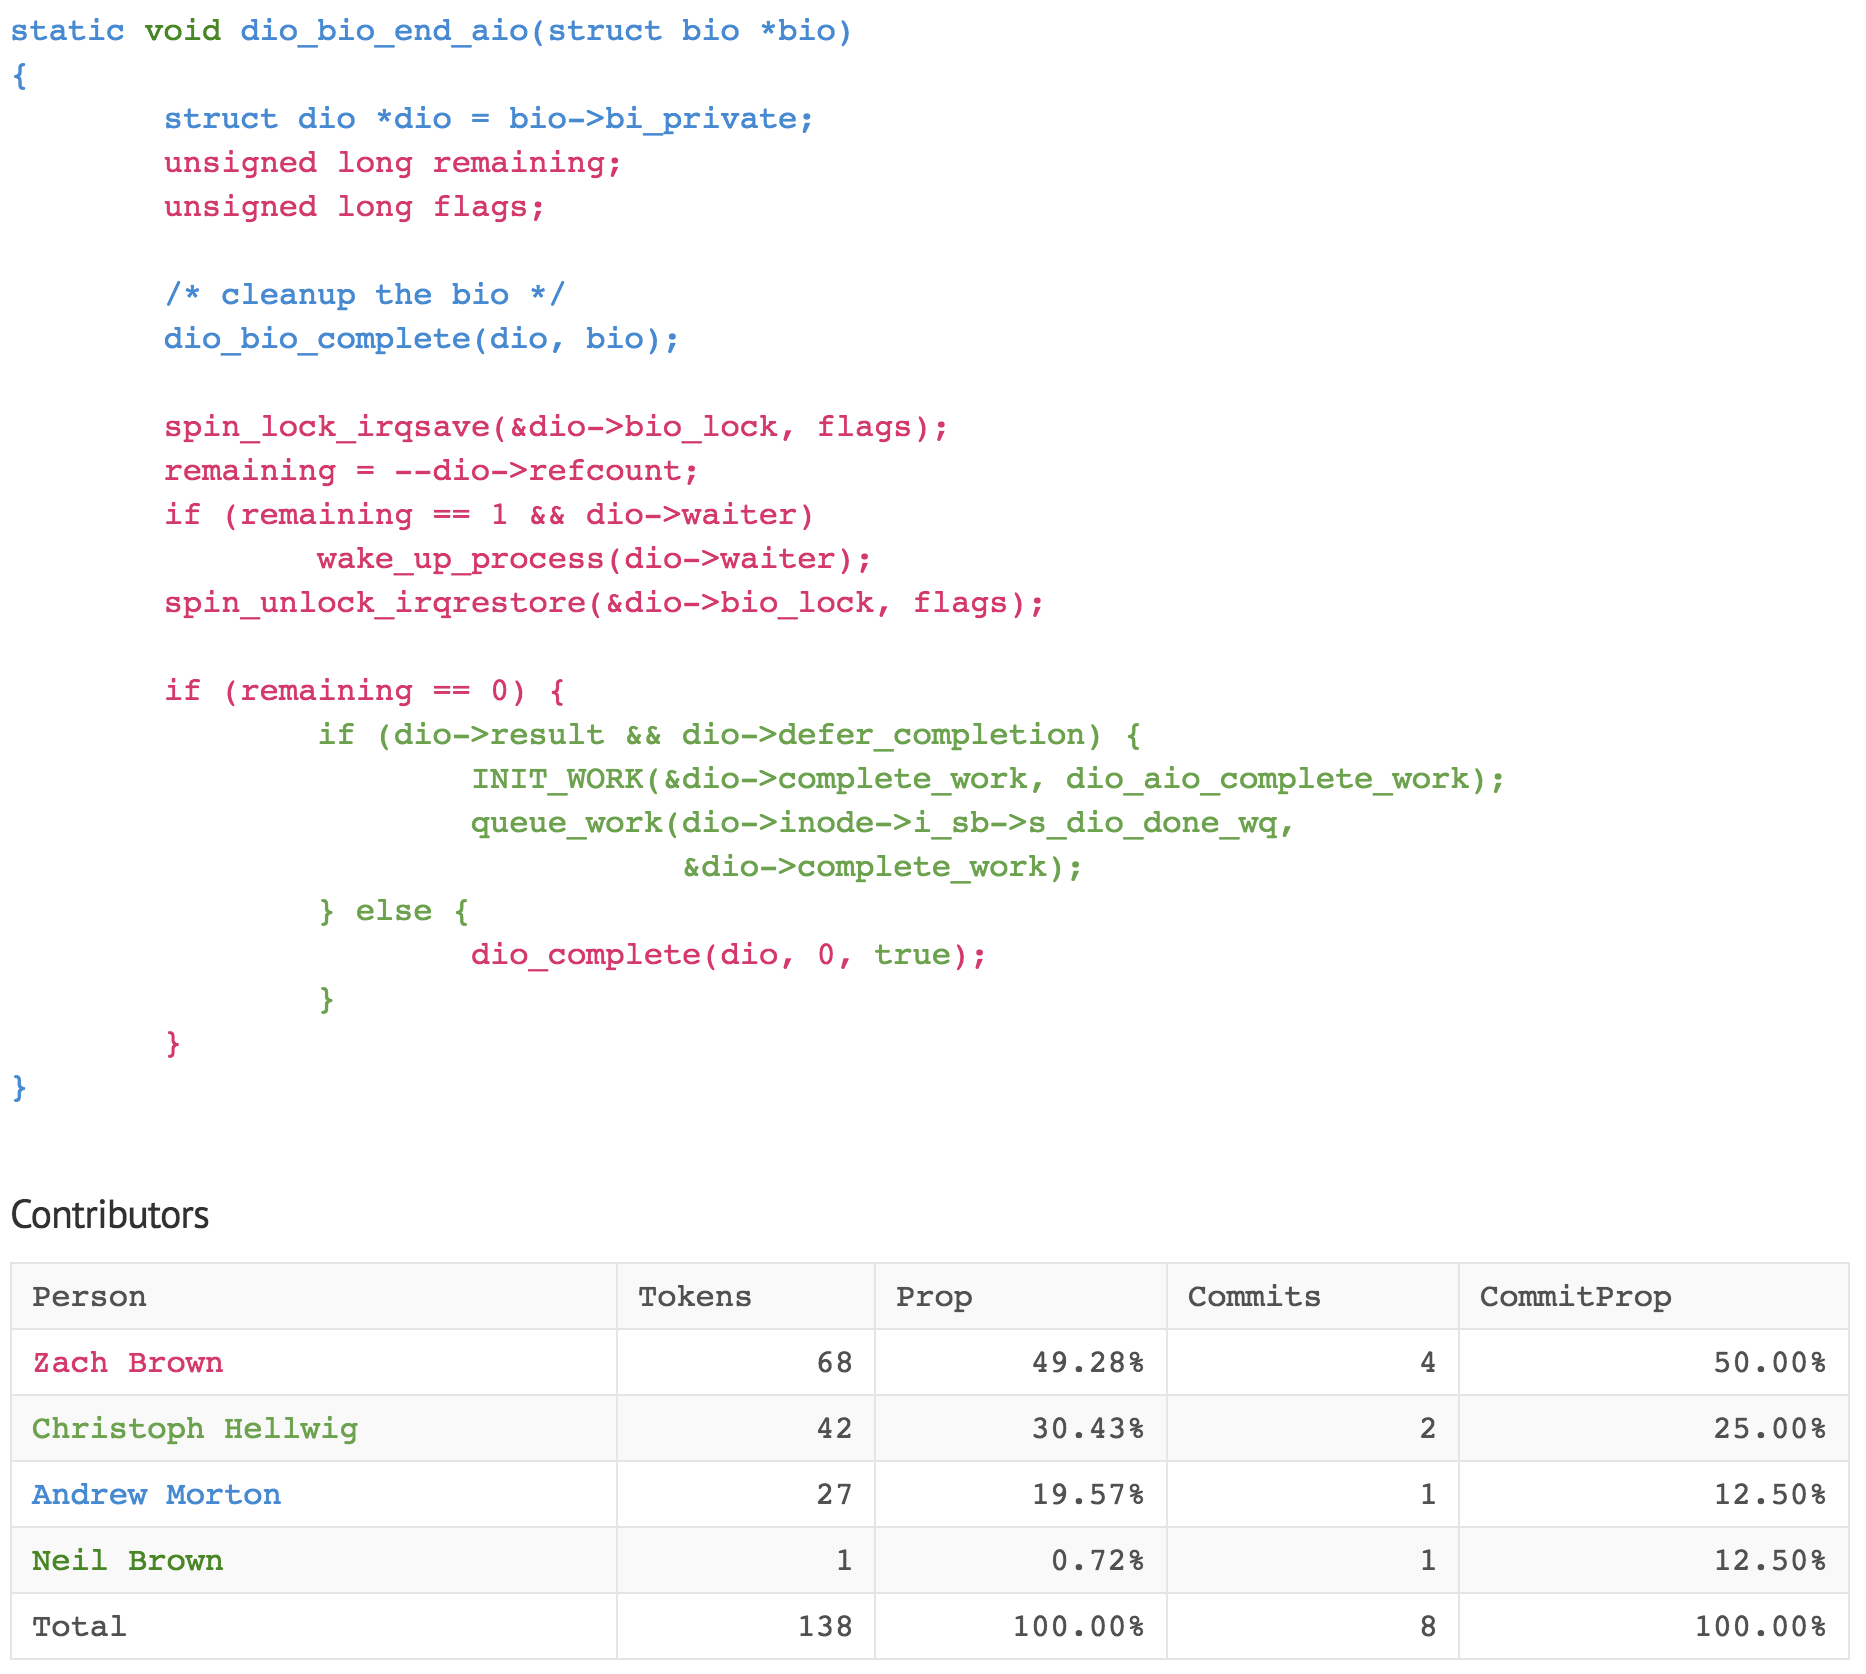
\includegraphics[width=0.8\textwidth]{cregit_code}
\caption{Tokenized source code as it appears on Cregit.}
\label{fig:cregit_code}
\end{figure}

\autoref{fig:cregit_code} shows tokenized linux code as it appears on the Cregit interface. In an effort to ease the access to email2git data, we decided to provide access to the matches through cregit. To this end, I modified the user interface to display a window containing all the available patches after clicking on a token, as shown in \autoref{fig:cregit_matches}. 

\begin{figure}[htb]
\centering
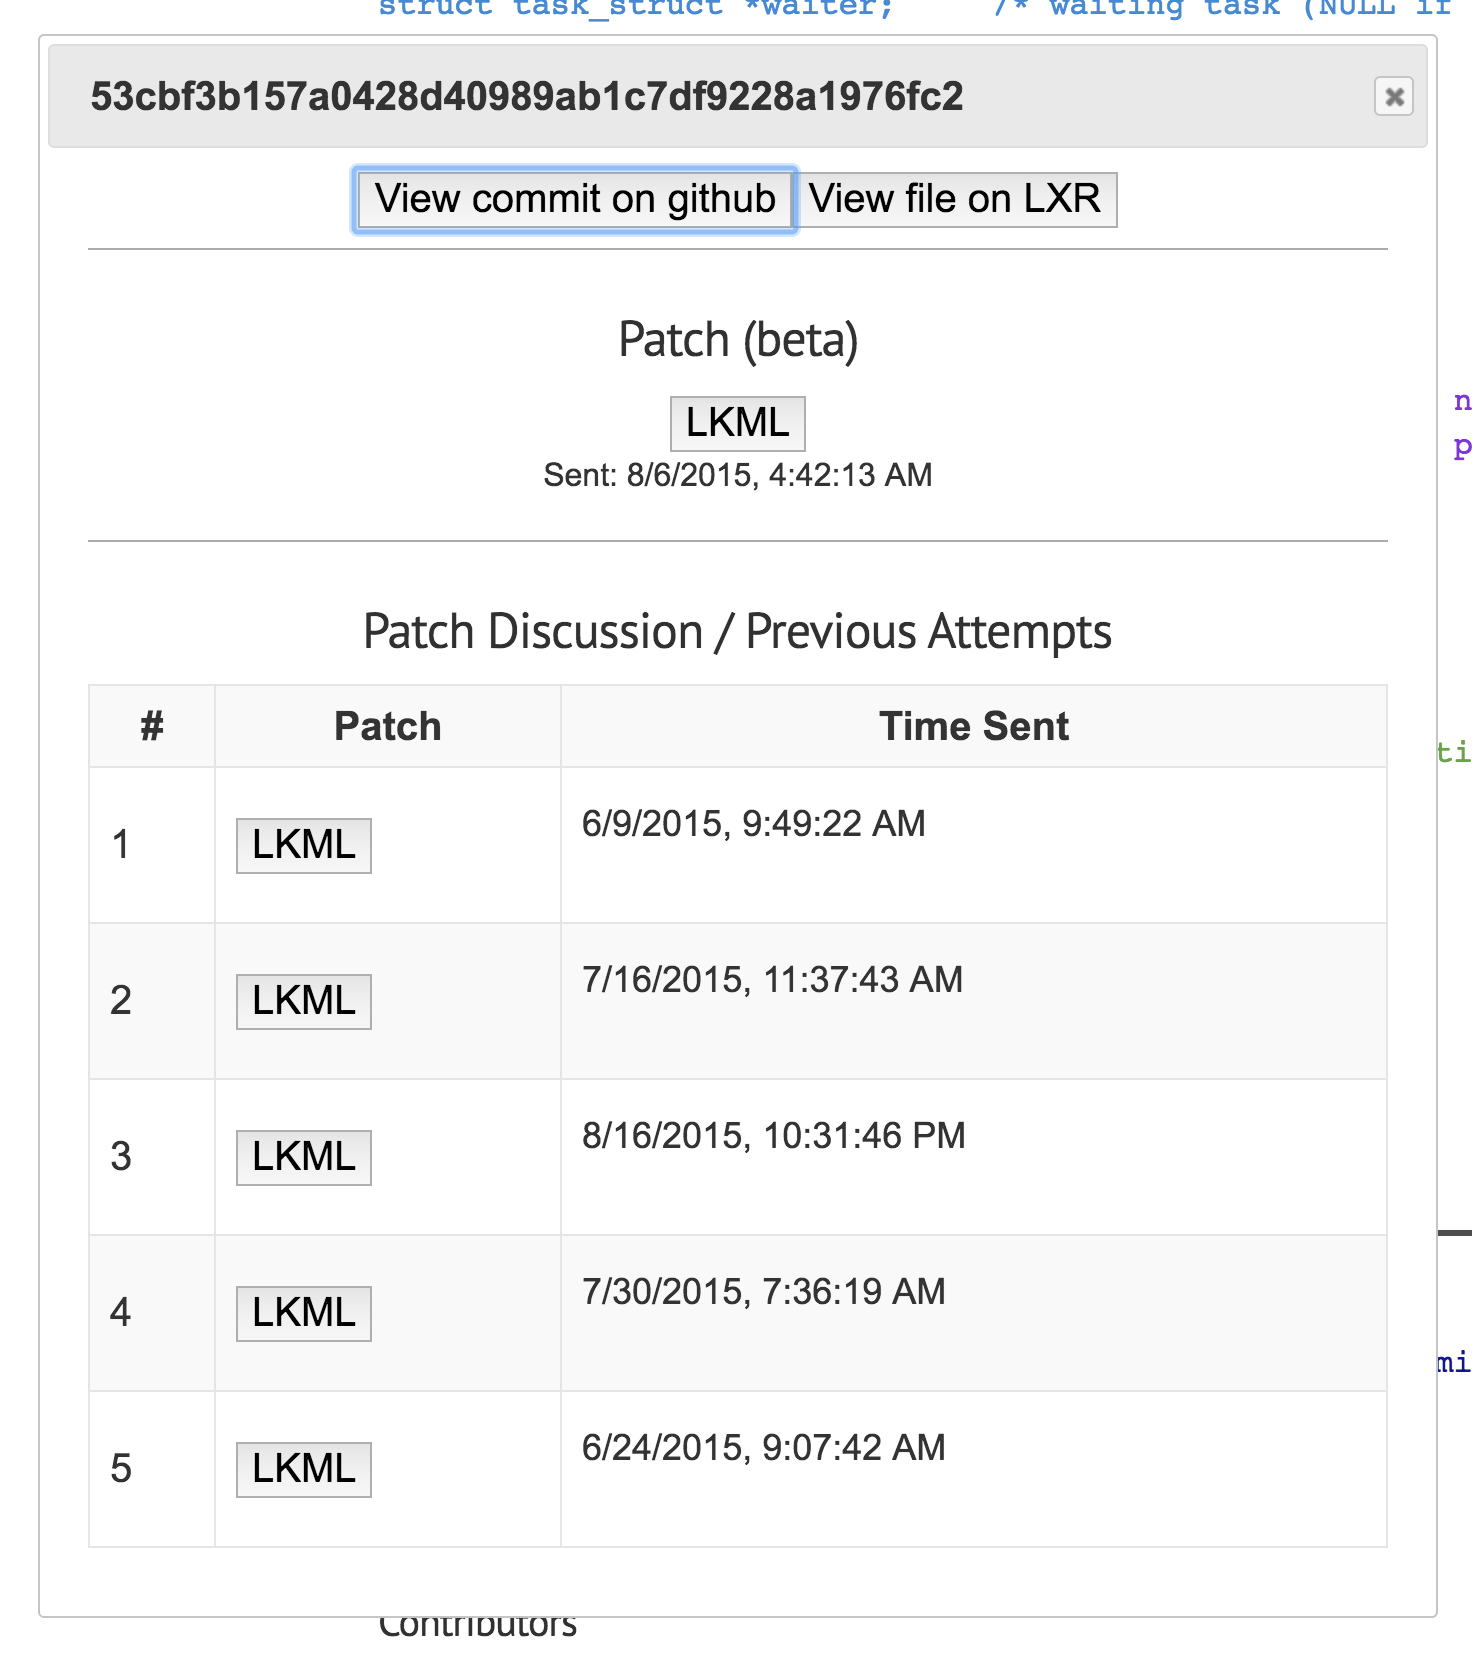
\includegraphics[width=3.5in]{cregit_matches}
\caption{Window containing the patches that introduced the commit associated with the clicked token}
\label{fig:cregit_matches}
\end{figure}




\subsection{Standalone Commit Lookup Tool}



Our second access point is a simple commit ID lookup tool. Although both platforms use the same UI and fetching mechanism to display the links to patchwork, the user experience is fundamentally different. On cregit, users navigate the interface by browsing the tokenized files as displayed in \autoref{fig:cregit_code}. Once the user clicks on a token, we display a window containing the links to the patches and conversation that introduced that token to the source code. Note that in this case, the user does not need to know the commit ID of the token of interest. The commit ID, which is necessary to retrieve the patches, is hard-coded in the html element containing the token. The HTML element containing a token looks like this:

\begin{lstlisting}[language=HTML]
<a onclick="return 
windowpopLinux('2ebda74fd6c9d3fc3b9f0234fc519795e23025a5')">
	include
</a>
\end{lstlisting}

The onclick event calls a function defined in a global javascript file: \texttt{cregit.js}. In the original implementation of the cregit interface, this function would open a new browser window and show the commit associated by the token on github. So I modified \texttt{cregit.js} to disable the "popup mechanism" and to instead use the commit ID to fetch the patchwork permalinks IDs from the server. The matches are stored as csv files named after the commit ID they are associated with on the server hosting the interface. The asyncronous request is done through Papaparse\footnote{\url{http://papaparse.com/}}, a powerful open source javascript library capable of downloading and parsing csv files from the client. The javascript code that generates the URLs from the permalinks and displays the new window lives in a callback function that executes after the request is complete. We were able to keep the "view commit on github" feature, by showing a button in the new window as displayed in \autoref{fig:cregit_matches}.  

On the standalone commit ID lookup page, \autoref{fig:email2git}, the mechanism is almost identical, but the user experience is completely different. Instead of clicking on a token, the user knows the commit ID in advance, as they might have encountered it while trying to fix a bug, or read a \texttt{git log} output. The user copies and pastes the commit ID in the search bar, and the match window appears with a list of dated links to patchwork order by time sent. The lookup page verifies whether the commit ID is a SHA-1 hash with the following regex:



\begin{lstlisting}
// removing white space
cid = cid.replace(/\s/g, '');

// validating input
if (!/\b[0-9a-f]{40,40}\b/.test(cid)){
    window.alert("The input should be a full 40-character SHA1 hash.");
    return;
}
\end{lstlisting}

\begin{figure}[htb]
\centering
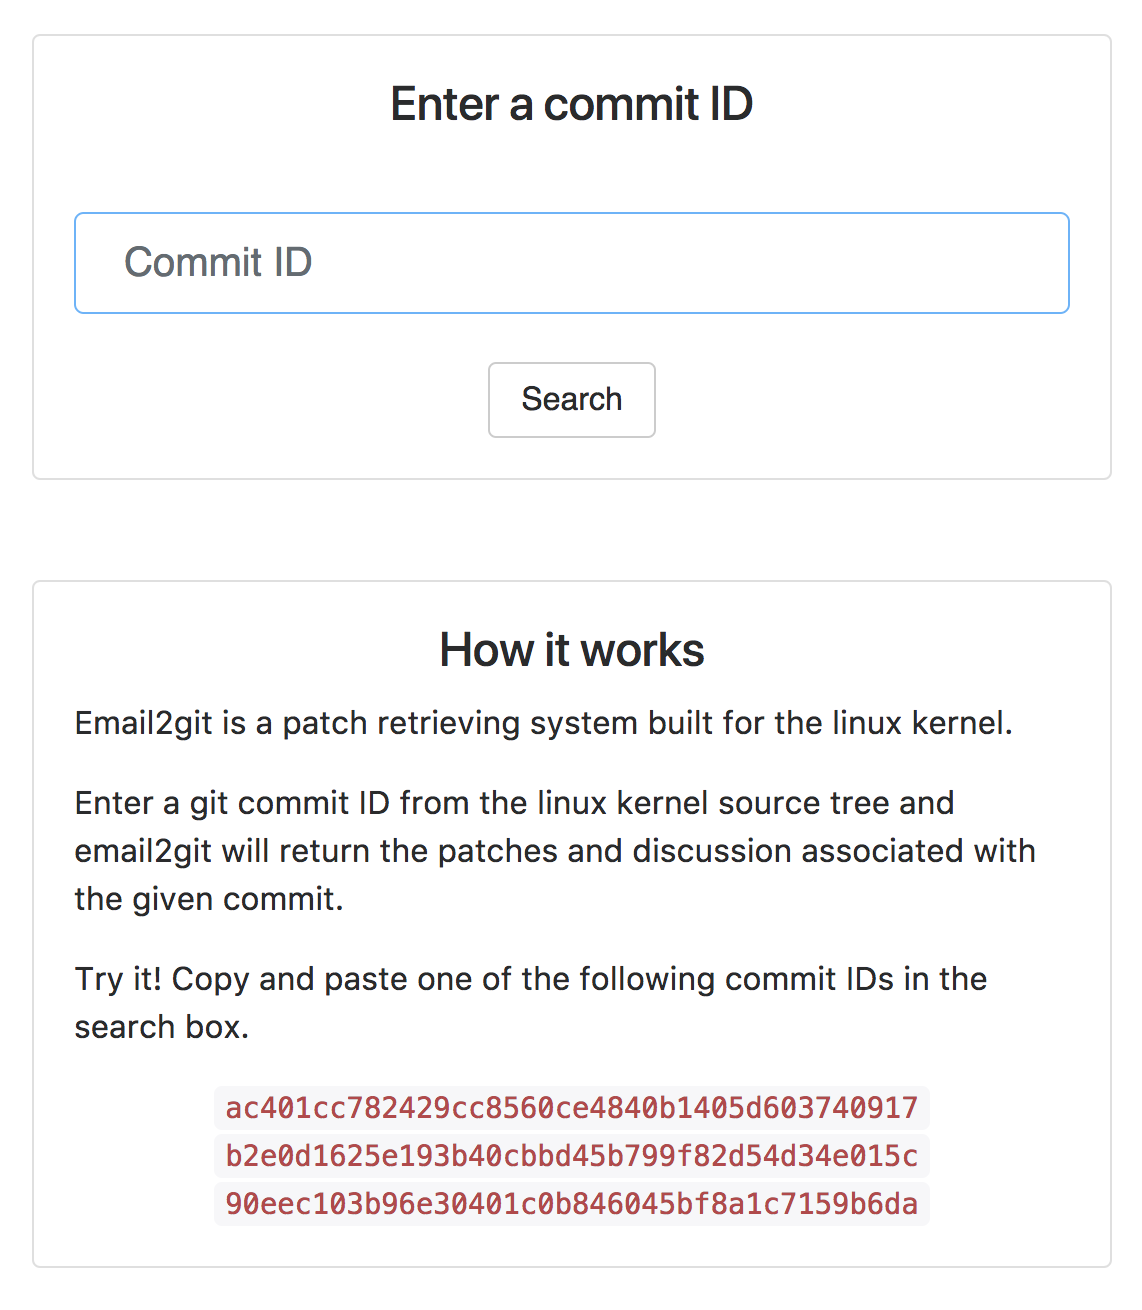
\includegraphics[width=3.5in]{email2git}
\caption{Standalone Commit ID Lookup Interface}
\label{fig:email2git}
\end{figure}



\section{Introducing Email2git to the Opensource Community}

We undertook various efforts to make our work more visible to the linux and open source community in general. The first effort was a blog post published on linux.com\footnote{\url{https://www.linux.com/blog/email2git-matching-linux-code-its-mailing-list-discussions}}. This blog post discusses email2git and its integration with cregit. This blog post was shared on Facebook and Twitter by the Linux Foundation and by other developers, which helped spread the word about our work. In addition to this blogpost, I gave a refereed talk at the Open Source Summit and the Linux Plumbers Conference in Los Angeles. This gave me the opportunity to give a demo, explain the underlying algorithm and finally discuss the project with developer and receive crucial feedback. An article\footnote{\url{https://lwn.net/Articles/734018/}} was published on LWN.net by Jake Edge following my talk. It explained the algorithm, the challenges faced, and mentioned some of the questions that were asked during the talk.


The linux developers feedback included the following points:
\begin{enumerate}
	\item \textbf{Including patch zero.} The patch zero is the email that introduces a multi-patch series. A multi-patch series is a large set of changes that is split over multiple emails. The patch zero contains information regarding the entirety of the patch series. Our current source of matches, lkml.kernel.org, uses patchwork 1.0, which did not track the patch zero. The patch zero feature was implemented in Patchwork 2.0.

	\item \textbf{Tracking Linux-next.} Linux-next is the branch used for integration testing. Developers would benefit from review discussions to help fix bugs that arised from integrating commits to Linux-next. In its current form, Email2git only contains matches for commits from the main tree, which means that Linux-next commits are not yet included.

	\item \textbf{Give credit to reviewers.} The \texttt{reviewed-by} tag is used to give credit to the developers that contributed during a patch review. However, some reviewers often do not receive the credit they deserve after contributing in reviews. Our tool could automate or help generate the \texttt{reviewed-by} tags.

	\item \textbf{Guidelines for more accurate matching.} A developer suggested the creation of a list of guidelines for developers to follow in their development process. These guidelines would promote the use of the built-in git features that use the email subject as commit-summary. If adopted by the community, those guidelines would increase the proportion of matches found. 
\end{enumerate}


\section{Evaluation}

To evaluate the current state of the tool, we look at the number of commits Email2git was able to match. Overall, the algorithm matched 57\% of the non-merge commits since 2009. We look at the proportion of commits matched in the largest subdirectories of the Linux Kernel source code. \autoref{fig:matched_proportions} presents these proportions. The proportion of matches found is unevenly spread across the different subdirectories of the Linux Kernel source code. For example, the \texttt{kernel} and \texttt{mm} directories have about \textbf{70\%} of their commits matched. On the other hand, the \texttt{net} directory only has \textbf{25\%} of their commits matched. This is mainly due to the absence of key mailing lists from our email dataset. One of these missing mailing lists is \texttt{netdev}, where many patches related to net development are sent. This is reflected in the low proportion of commits matched in the \texttt{net} subdirectory. 


\begin{figure}[htb]
\centering
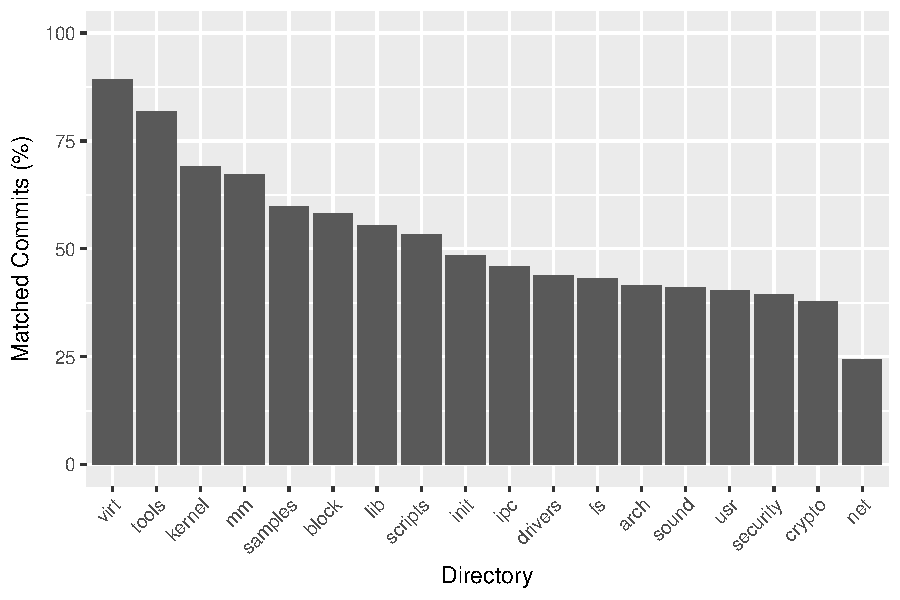
\includegraphics[width=5in]{plots/matched_commits_dir}
\caption{Percentage of matched commits in Linux subdirectories, from 2009 to the time of writing this thesis}
\label{fig:matched_proportions}
\end{figure}

Furthermore, we can break down the matches by the stage of the algorithm that generated them. The first phase of the algorithm, which uses the email subject, finds about \textbf{95\%} of the final set of matches. The second part of the algorithm, which uses the author and filename based matching, finds \textbf{5\%} of the final matches. It is important to note that the second phase of the algorithm is exposed to less commits than the first phase. The commits matched by the first phase are removed from the dataset before starting the second phase. This implies that the second phase will inherently find less matches than the first phase. We tested the performance of the line-based algorithm (both author and filename) on a subset of commit and patches to understand its performance. The algorithm found a \textit{correct} match for \textit{26\%} of the analyzed commits.



Finally, we are running an analytics script on the server hosting the matches to understand the usage of the data and to know the proportion of requested commit IDs are not matched. Removing the whitespace and assuring the validity of the string ensures the accuracy of these statistics, by reducing the number of failed requests due to a poorly formatted commit ID.

\begin{figure}[htb]
\centering
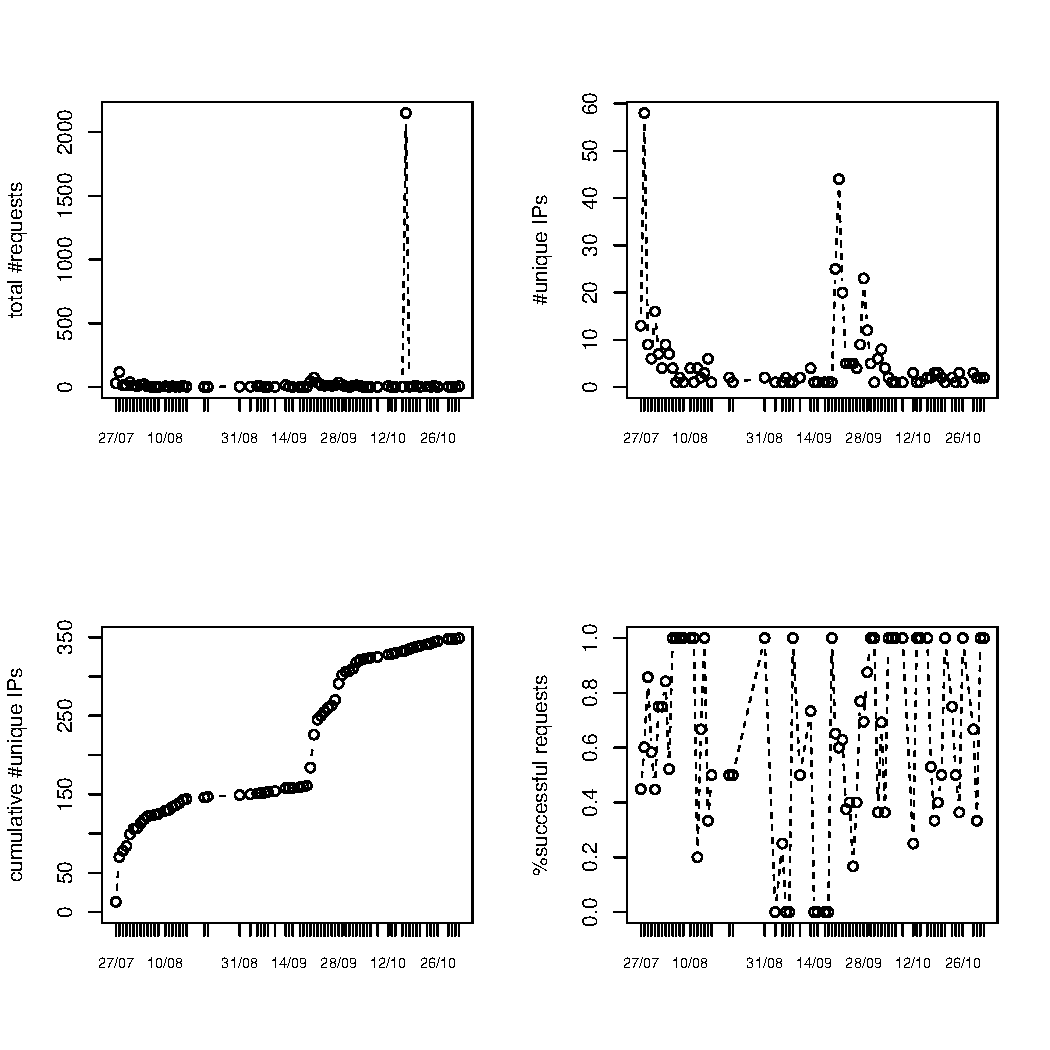
\includegraphics[width=5in]{analytics}
\caption{Plots created from the analytic}
\label{fig:analytics}
\end{figure}

\autoref{fig:analytics} displays the plots created by the analytics script running on the server. We observe two peaks in number of unique IP addresses at two different moments: at the end of July and in mid September. The former date corresponds to the day we introduced Email2git in a blogpost on linux.com and the latter corresponds to the talk I gave at the Open Source Summit North America in Los Angeles. 

\section{Conclusion}

We leveraged the lessons learned from Srcmap while creating Email2git. The purpose of Email2git was to answer a complain coming from multiple developers and maintainers: the difficulty of finding an email discussion about patches that were eventually integrated in the Linux Kernel. Understanding the Linux community allowed us to better introduce our tool when we released it, as explained in Chapter 4. Moreover, the data acquired in the implementation of Email2git served as one of the metrics used by our expertise model as explained in chapter 5.


% \alex{email2git successful, developers showed interest, }

% \alex{intention to pursue development, features to implement. patchwork with more mailing lists. Pipeline. linux next}
